\documentclass[12pt]{article}

\usepackage{graphicx}
\usepackage{paralist}
\usepackage{amsfonts}
\usepackage{hyperref}
\usepackage{listings}
\usepackage{subfig}
\usepackage{float}

\oddsidemargin 0mm
\evensidemargin 0mm
\textwidth 160mm
\textheight 200mm
\renewcommand\baselinestretch{1.0}

\pagestyle {plain}
\pagenumbering{arabic}
\newcounter{stepnum}

\title{Course Project}
% \author{Hyosik Moon}
\author{
  Moon, Hyosik
  }

\begin {document}

\maketitle

\section{Required}

\begin{itemize}
\item \textbf{Main objective of the analysis} \\
HELP International have been able to raise around \$ 10 million. Now the CEO of the NGO needs to decide how to use this money strategically and effectively. So, CEO has to make decision to choose the countries that are in the direst need of aid. Hence, your Job as a Data scientist is to categorise the countries using some socio-economic and health factors that determine the overall development of the country. Then you need to suggest the countries which the CEO needs to focus on the most.\\

I will categorise the countries into some groups and suggest the countries in the poorest group. Let's find which countries belong to the poorest group.


\item \textbf{Brief description of the data set} \\
There are 167 rows which are countries and 10 columns explaining the countries' information such as 
Columns0: country --- Description: Name of the country
Columns1: child\_mort --- Description: Death of children under 5 years of age per 1000 live births
Columns2: exports --- Description: Exports of goods and services per capita. Given as \%age of the GDP per capita
Columns3: health --- Description: Total health spending per capita. Given as \%age of GDP per capita
Columns4: imports --- Description: Imports of goods and services per capita. Given as \%age of the GDP per capita
Columns5: Income --- Description: Net income per person
Columns6: Inflation --- Description: The measurement of the annual growth rate of the Total GDP
Columns7: life\_expec --- Description: The average number of years a new born child would live if the current mortality patterns are to remain the same
Columns8: total\_fer --- Description: The number of children that would be born to each woman if the current age-fertility rates remain the same.
Columns9: gdpp --- Description: The GDP per capita. Calculated as the Total GDP divided by the total population.
(Figure \ref{data})

\begin{figure}[H]
  \centering
  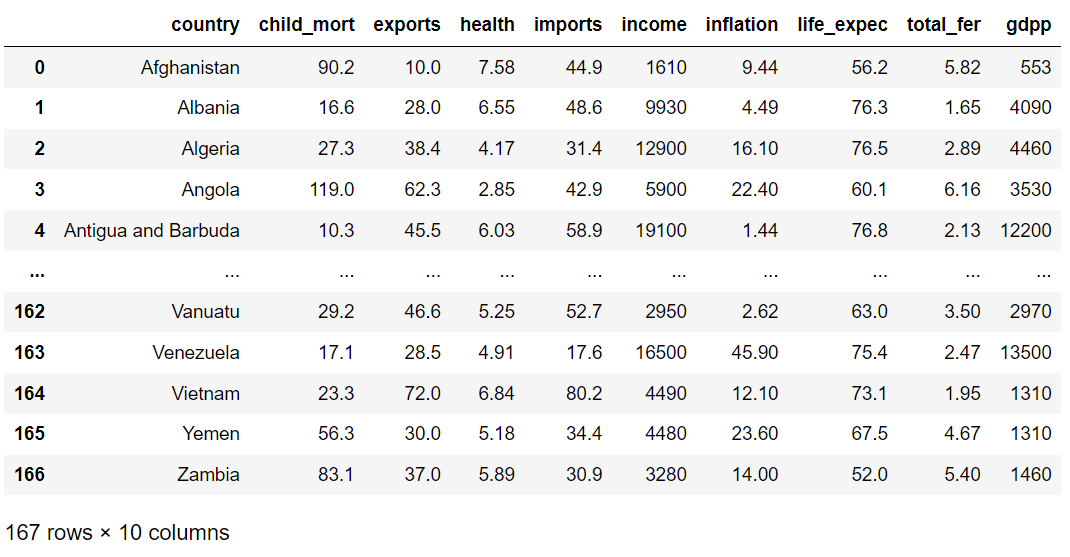
\includegraphics[width=0.9\textwidth]{figures/data.png}
  \caption{Original data}\label{data}
\end{figure}

\item \textbf{Brief summary of data exploration}
In order to cluster the data accurately we need to explore and preprocess. For the accurate distance calculation between data, I preprocessed them according to the following steps: Data types - Remove - Skew - Scaling - Pairplot.
  \begin{enumerate}
    \item 1. Data types 
      I changed income and gdpp data types from int to float in order to calculate closeness between cluster later.
    \item 2. Remove
      We will cluster countries, so we don't need the country column and I also deleted NaN values in data.
    \item 3. Skew 
      Check the skewness of the columns and take log1p if the value of skewness is higher than 0.75.
    \item 4. Scaling
      I used MinMaxScaler to normalize them as an equal size. Picture \ref{datap} is the processed data.
      \begin{figure}[H]
        \centering
        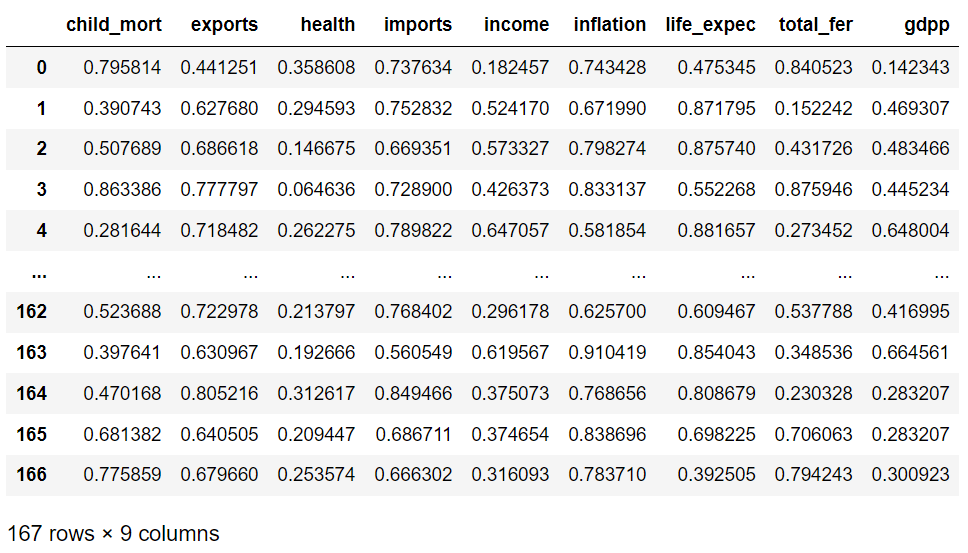
\includegraphics[width=0.9\textwidth]{figures/datap.png}
        \caption{Processed data}\label{datap}
      \end{figure}
    \item 5. Pairplot
      Picture \ref{pplt} is the processed data' pairplot.
      \begin{figure}[H]
        \centering
        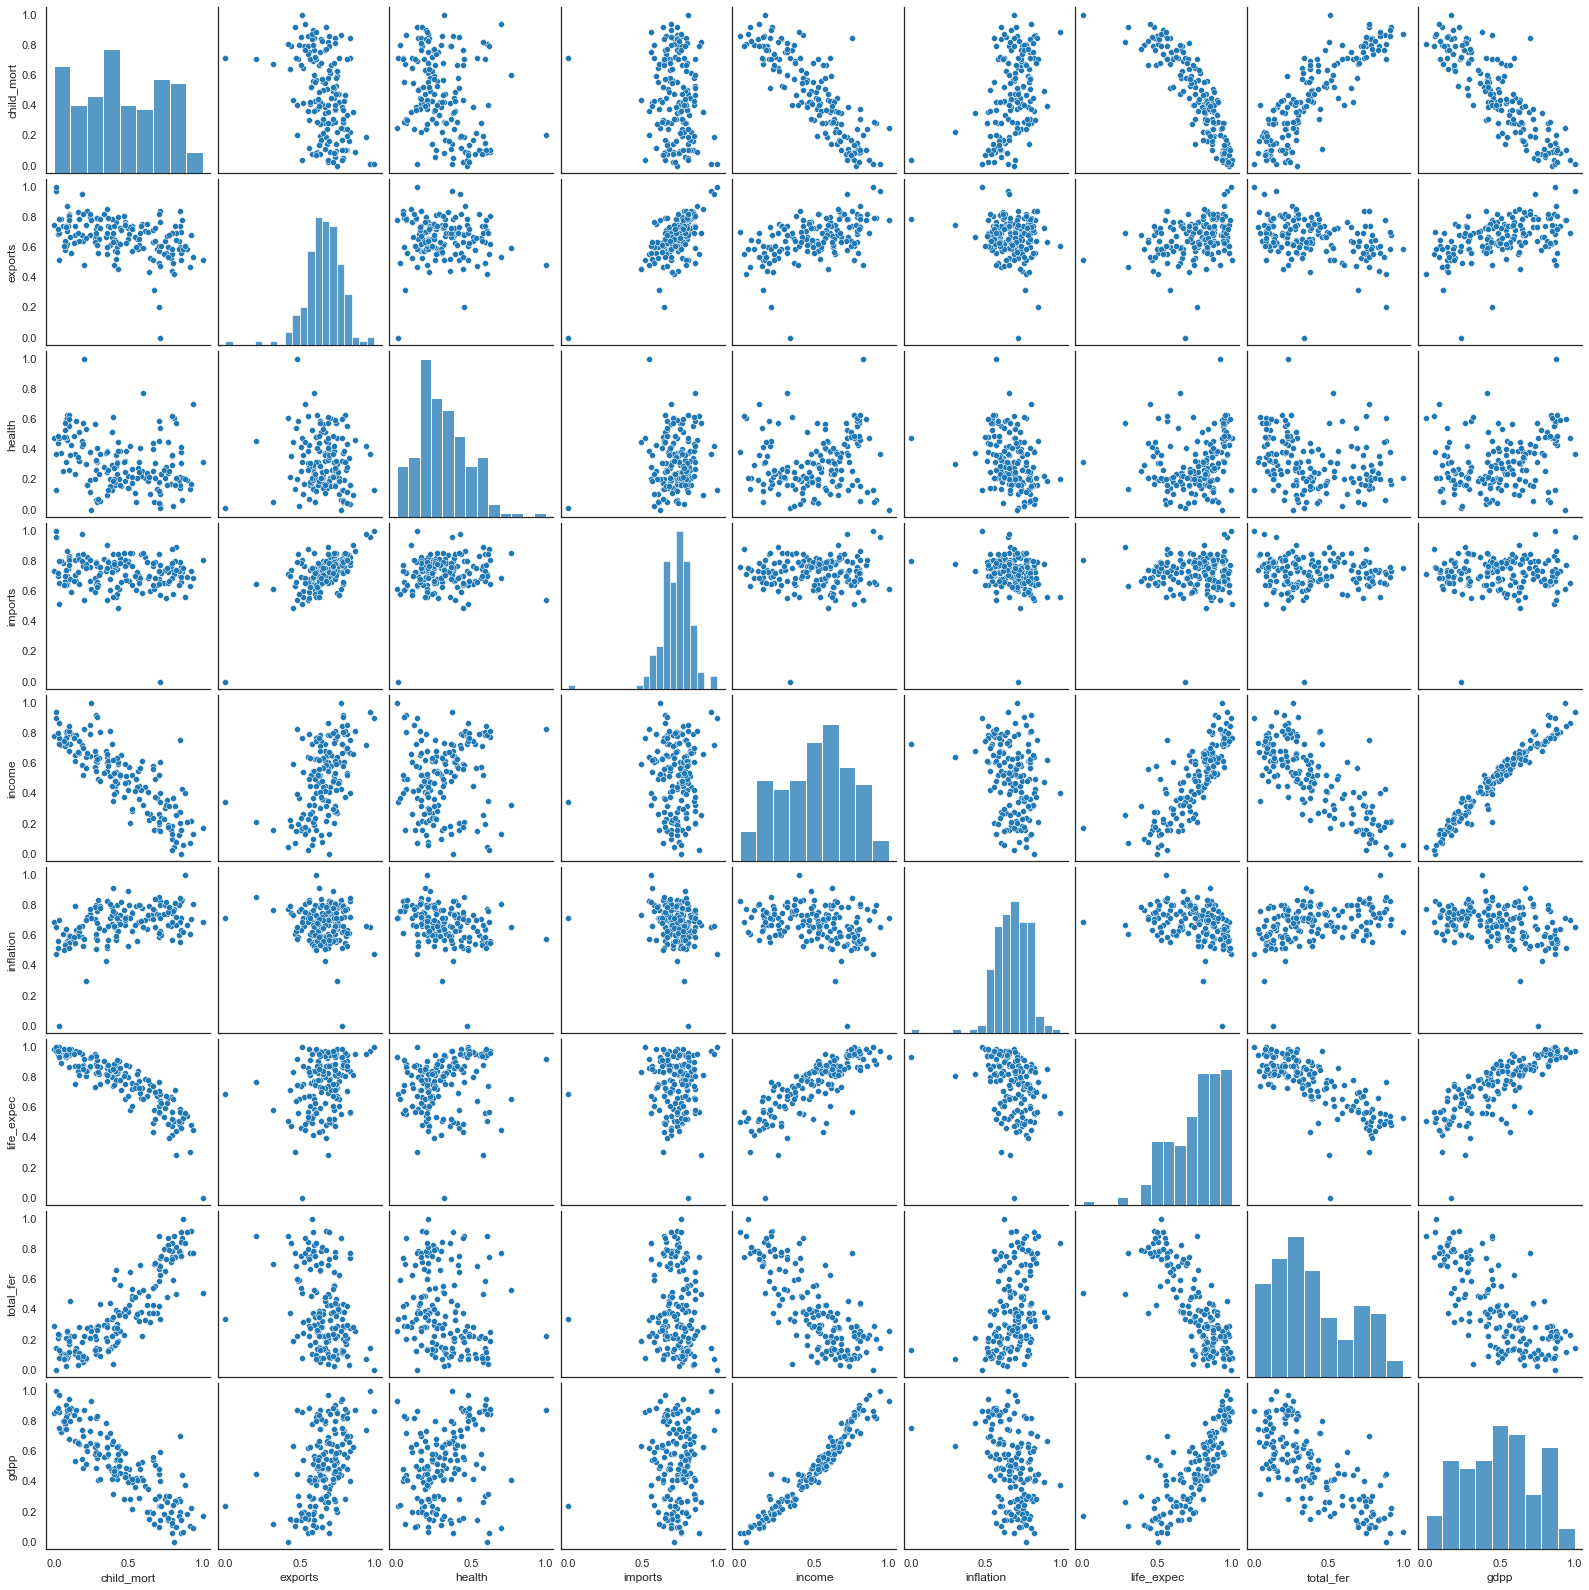
\includegraphics[width=0.9\textwidth]{figures/pplt.png}
        \caption{Pairplot of the data}\label{pplt}
      \end{figure}
  \end{enumerate}

\item \textbf{Summary of training at least three models} I implemented three different clustering algorithms which are `K-Means, Hierarchical Agglomerative Clustering, and Non-negative '.
    \begin{enumerate}
      \item K-Means. I tested the kmeans algorithm with 10 different K values to find the optimal one. I found the optimal K=4, by using the elbow method (Figure \ref{kmeans}).
      \begin{figure}[H]
        \centering
        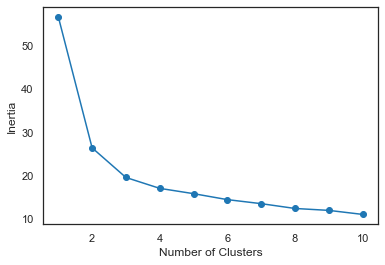
\includegraphics[width=0.9\textwidth]{figures/kmeans.png}
        \caption{K-Means' inertia plot}\label{kmeans}
      \end{figure}

      Figure \ref{clusters} is the clustering results, so we can know that 1-cluster is the poorest group. So, we need to support the countries in 1-cluster first. 
      \begin{figure}[H]
        \centering
        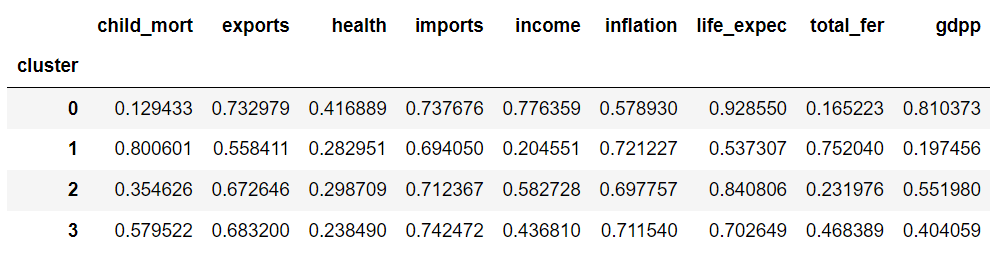
\includegraphics[width=0.9\textwidth]{figures/clusters.png}
        \caption{K-means Clustering result}\label{clusters}
      \end{figure}

      The countries in 1-cluster are that: \\
      cluster               country\\
      1                     Burundi\\
      1                     Liberia\\
      1            Congo, Dem. Rep.\\
      1                       Niger\\
      1                Sierra Leone\\
      1                  Madagascar\\
      1                  Mozambique\\
      1    Central African Republic\\
      1                      Malawi\\
      1                     Eritrea\\
      1                        Togo\\
      1               Guinea-Bissau\\
      1                 Afghanistan\\
      1                      Gambia\\
      1                      Rwanda\\
      1                Burkina Faso\\
      1                      Uganda\\
      1                      Guinea\\
      1                       Haiti\\
      1                    Tanzania\\
      1                        Mali\\
      1                  Tajikistan\\
      1                       Benin\\
      1                     Comoros\\
      1                        Chad\\
      1                       Kenya\\
      1                     Myanmar\\
      1                     Senegal\\
      1                    Pakistan\\
      1                     Lesotho\\
      1                  Mauritania\\
      1               Cote d'Ivoire\\
      1                       Ghana\\
      1                    Cameroon\\
      1                       Yemen\\
      1                      Zambia\\
      1                       Sudan\\
      1                    Kiribati\\
      1                     Nigeria\\
      1                      Angola\\
      1                 Timor-Leste\\

      \item AgglomerativeClustering. I implemented AgglomerativeClustering algorithm with 4 clusters (Figure \ref{agglom}). We can know that 3-cluster is the poorest group.
      \begin{figure}[H]
        \centering
        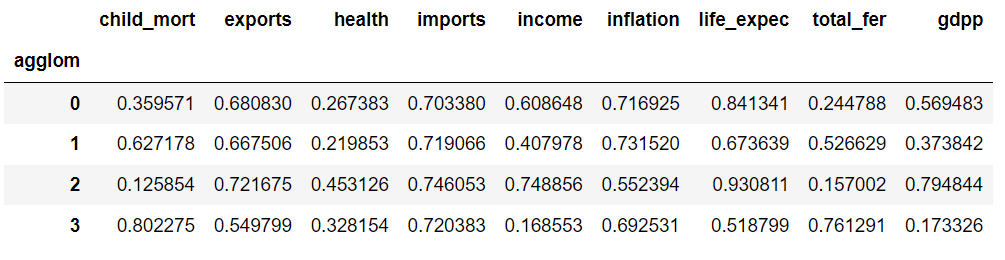
\includegraphics[width=0.9\textwidth]{figures/agglom.png}
        \caption{AgglomerativeClustering}\label{agglom}
      \end{figure}

      The countries in 3-cluster are that: \\
      cluster               country\\
      3                     Burundi\\
      3                     Liberia\\
      3            Congo, Dem. Rep.\\
      3                       Niger\\
      3                Sierra Leone\\
      3                  Madagascar\\
      3                  Mozambique\\
      3    Central African Republic\\
      3                      Malawi\\
      3                     Eritrea\\
      3                        Togo\\
      3               Guinea-Bissau\\
      3                 Afghanistan\\
      3                      Gambia\\
      3                      Rwanda\\
      3                Burkina Faso\\
      3                      Uganda\\
      3                      Guinea\\
      3                       Haiti\\
      3                    Tanzania\\
      3                        Mali\\
      3                       Benin\\
      3                     Comoros\\
      3                        Chad\\
      3                       Kenya\\
      3                     Senegal\\
      3                    Pakistan\\
      3                     Lesotho\\
      3                    Cameroon\\
      3                    Kiribati\\
      3       Micronesia, Fed. Sts.\\
      3                 Timor-Leste\\

      \item Non-negative Matrix Fatorization. This is dimensionality reduction method. I reduced the dimensionality to 4. Figure \ref{variance} is the variance result of the each dimension. I clustered the countries based on the highest variance. Thus, countries were categorized into 3 groups (Figure \ref{nmf}). We can know that 3-cluster is the poorest group.
      \begin{figure}[H]
        \centering
        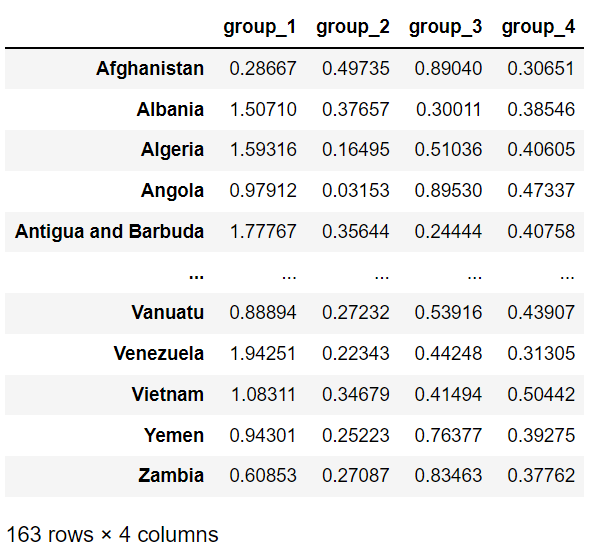
\includegraphics[width=0.9\textwidth]{figures/variance.png}
        \caption{Variance of NMF}\label{variance}
      \end{figure}

      \begin{figure}[H]
        \centering
        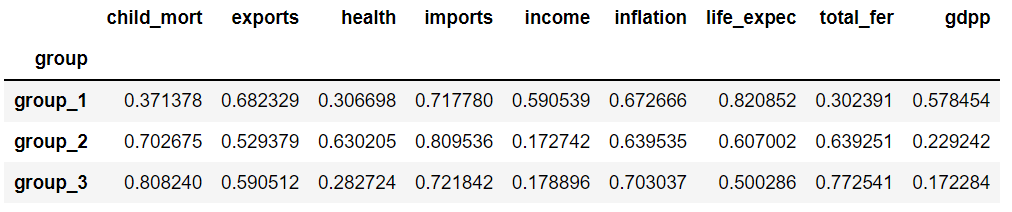
\includegraphics[width=0.9\textwidth]{figures/nmf.png}
        \caption{Non-negative Matrix Fatorization clustering result}\label{nmf}
      \end{figure}

      The countries in 3-cluster are that: \\
      cluster                      country\\
      group\_3                     Burundi\\
      group\_3            Congo, Dem. Rep.\\
      group\_3                       Niger\\
      group\_3                Sierra Leone\\
      group\_3                  Madagascar\\
      group\_3                  Mozambique\\
      group\_3    Central African Republic\\
      group\_3                      Malawi\\
      group\_3                     Eritrea\\
      group\_3                        Togo\\
      group\_3               Guinea-Bissau\\
      group\_3                 Afghanistan\\
      group\_3                      Gambia\\
      group\_3                Burkina Faso\\
      group\_3                      Uganda\\
      group\_3                      Guinea\\
      group\_3                       Haiti\\
      group\_3                    Tanzania\\
      group\_3                        Mali\\
      group\_3                       Benin\\
      group\_3                     Comoros\\
      group\_3                        Chad\\
      group\_3                       Kenya\\
      group\_3                     Senegal\\
      group\_3                     Lesotho\\
      group\_3                  Mauritania\\
      group\_3               Cote d'Ivoire\\
      group\_3             Solomon Islands\\
      group\_3                       Ghana\\
      group\_3                    Cameroon\\
      group\_3                      Zambia\\

    \end{enumerate}

\item \textbf{Explanation of your final model}
Based on the three algorithms, top-10 poorest countries are almost same but in the case of nmf some of poorest countries are not included such as 'Liberia' and it clustered the countries into 3 groups which are more broad. Thus, I think K-means (or HAC) is the final model that I choose.

\item \textbf{Summary Key Findings and Insights}
Although NMF shows a little bit different results compared to K-means and HAC, the result is almost same. If I have to save resources I think NMF will be the best model. And we need to help top-10 poorest countries such as \\
1                     Burundi\\
1                     Liberia\\
1            Congo, Dem. Rep.\\
1                       Niger\\
1                Sierra Leone\\
1                  Madagascar\\
1                  Mozambique\\
1    Central African Republic\\
1                      Malawi\\
1                     Eritrea\\
.

\item \textbf{Suggestions for next steps}
It will be interesting to analyse the reason why the NMF clusters our data into 3 groups not 4 groups which means the highest variance belonged only into 3 groups. Does it mean that we can reduce the principle components into 3 not 4?

\end{itemize}

\end {document}